\documentclass{beamer}
\usepackage[utf8x]{inputenc}
\usepackage[czech]{babel}
\usetheme[pageofpages=of,% String used between the current page and the
                         % total page count.
          bullet=circle,% Use circles instead of squares for bullets.
          titleline=true,% Show a line below the frame title.
	  titlepagelogo=opensuse,
          alternativetitlepage=true,% Use the fancy title page.
          ]{Torino}

\setbeamerfont{title}{series=\bfseries,size=\LARGE}
\author{Tom\'{a}\v{s} Chv\'{a}tal\newline {\small openSUSE Team}}
\title{Dealing with toxic personalities}
\date{2013/07/19}

\begin{document}

\begin{frame}[t,plain]
\titlepage
\end{frame}

\section{Introduction}

\begin{frame}[t]{Who the hell is Tomáš Chvátal}
	\begin{itemize}
	\item SUSE Employee since 2011 (QA, openSUSE)
	\item Packager of Libreoffice and various other for openSUSE
	\item openSUSE promoter and volunteer
	\item Gentoo developer since fall 2008 and Council member since 2010
	\end{itemize}
\end{frame}

\section{Contribution process}

\begin{frame}{Contribution cycle}
	\begin{figure}
	\includegraphics[width= 0.8\linewidth]{contribution-process.png}
	\end{figure}
\end{frame}

\section{Describing toxic person}

\begin{frame}[t]{Finding a toxic person}
	\begin{itemize}
	\item Use of personal attacks and insults
	\item Atacker mostly tries to focus on the less-powerfull (newcommers/etc.) members of the community
	\item People are demotivated by having to work with such person
	\item Look for cycles and patterns, each of us can have rough day
	\end{itemize}
\end{frame}

\begin{frame}{What is NOT a toxic person}
	\begin{center}
	\textbf{Someone who disagrees with you on technical level}
	\end{center}
\end{frame}

\begin{frame}{How hard it is to redeem credit}
	\begin{center}
	\textbf{For one bad action you need 5+ positive actions to get even}
	\end{center}
\end{frame}

\section{Outcome from toxic person actions}

\begin{frame}[t]{What happens to targeted person}
	\begin{itemize}
	\item Becomes less commited - 78\%
	\item Decreases quality of contributions - 39\%
	\item Loses time avoiding - 63\%
	\item Loses time worrying - 80\%
	\item Quits - 25\%
	\item \textbf{Witnesses} quit - 25\%
	\end{itemize}
\end{frame}

\begin{frame}[t]{What happens to your project}
	\begin{itemize}
	\item Reduction of cooperation between developers
	\item Reduced contribution from outer project and people (forks, upstream)
	\item Atracting more toxic people rather than the best people
	\item Alienating women because they rather avoid rude environments
	\end{itemize}
\end{frame}

\section{How to protect people and project}

\begin{frame}{Fixing recruiting process}
	\begin{center}
	Technical skills are not everything. One has to ensure there are some social skills in the person too.
	\end{center}
\end{frame}

\begin{frame}[t]{Improving interproject communication}
	\begin{itemize}
	\item Have conferences
	\item Do regular team meetings where people can socialize
	\end{itemize}
	\vspace{0.8cm}
	\begin{center}
	This all is done to help people realize that on the other side of the wire there is real living and breathing person.
	\end{center}
\end{frame}

\begin{frame}[t]{Create team to handle community relations}
	\begin{itemize}
	\item You need to have body where to complain if someone is unjust
	\item The actions must be fast paced and just
	\item Nothing good comes out of a four month discussion about some activity (complainer will be long gone at that time) or day 1 overreaction
	\end{itemize}
\end{frame}

\begin{frame}[t]{Keep your standards}
	\begin{itemize}
	\item Require great standards from everyone
	\item Provide Code of Conduct or some form of Ethic code
	\end{itemize}
\end{frame}

\section{Reading}

\begin{frame}{Reading}
	\begin{figure}
	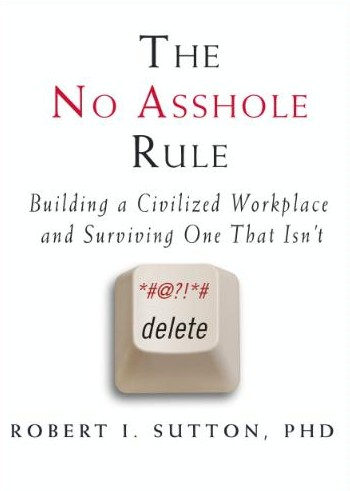
\includegraphics[width= 0.4\linewidth]{The_No_Asshole_Rule.jpg}
	\end{figure}
\end{frame}

\section{Thanks}

\begin{frame}{Suse is hiring}
	\begin{figure}
	
\includegraphics[width= 0.8\linewidth]{suse_hiring.png}
	\end{figure}
\end{frame}

\begin{frame}{Thanks}
	\begin{center}
	Thank you for your attention.
	\end{center}
\end{frame}

\end{document}

